


\section{Multi-View Framework}\label{sec:architecture}

Our proposed software engineering methodology for semantically aligned DTs is grounded in a multi-view framework depicted in Figure~\ref{fig:Tailoring:PTView2DTView}. In this context, a system view, or PT-view, is a formal model that captures a specific concern of the PT such as timing, functional, or safety constraints through a formal model. By separating concerns into views, the framework enables concern-specific reasoning while maintaining consistency across abstraction levels. Any implementation of the PT must therefore refine these views; that is, exhibit only behaviors permitted by them, preserving all their properties.

The DT is the artifact that enables prediction, monitoring, optimization, and adaptation throughout the PT's operational lifetime. The development of the DT is guided by the DT-specific views, which capture the subset of the corresponding PT-view relevant to the aforementioned tasks. Multiple DT views may correspond to a single PT view and each must be shown to be a refinement of it, ensuring that they faithfully capture it, to ensure the specification-level coherence of the DT with respect to the PT. Similarly to the PT, the DT must also be shown to refine its DT-specific views.


We aim at establishing semantic alignment between the DT and the PT at the view level, rather than at the implementation level.  Views are the authoritative design-time artifacts in MBSE and the natural locus of formal reasoning: implementations are generated from or refine them by construction, so view-level alignment propagates to the deployed system without additional proof obligation, independently of implementation technology, vendor, or instance. The multi-view structure further allows each DT-view to be aligned independently with its corresponding PT-view, with overall alignment composed from the parts. Finally, views are abstract and technology-agnostic, and are the artifacts exposed across organizational boundaries in federated settings such as Gaia-X, making view-level alignment the only kind establishable between independently developed twins.
%The ultimate goal of the framework is to ensure that the DT is a trustworthy representation of the PT, and that decisions based on the DT are sound with respect to the PT. To this end, the framework requires that the DT and the PT are semantically aligned, i.e.,
%that they agree on the semantics at data and behavior level.
%Following the paradigm of MBSE, we aim to establish alignment at
%the view level rather than at the implementation level. This choice is
%motivated by the following considerations. 

%First, views are the authoritative design-time artifact in MBSE and the natural locus of formal reasoning, with implementations generated from or refining them by construction. View-level alignment thus propagates to implementations through standard refinement, sufficient to ensure semantic alignment of the deployed system. Second, this propagation is independent of implementation technology, vendor, or instance: a single view-level alignment guarantee covers all implementations of the same view, whether produced by different vendors, deployed in parallel across environments, or replaced over time as the implementation evolves. Third, the multi-view structure of MBSE allows each DT-view to be aligned independently with the corresponding PT-view, with overall DT-PT alignment composed from the parts and parametric in the formalism used by each view, rather than committed to a uniform implementation-level semantics. Finally, views are abstract and technology-agnostic, and are the artifacts exposed across organizational boundaries in federated settings such as Gaia-X, making view-level alignment the only kind establishable between
%independently developed twins. 
%
%%Finally, 
%
%
%view-level alignment
%composes with refinement of the supporting domain knowledge
%(Theorem~\ref{thm:domain-refinement}), so iterative co-evolution of
%$\VPT$, $\VDT$, and $\DomainKnowledge$ preserves previously
%established alignment results without requiring re-verification.
%\end{}






%Following the paradigm of MBSE, we aim to establish alignment at the view level, which 







%In order to enable run-time monitoring and decision-making, the DT and the PT must be shown to be semantically aligned. While the specification-level correctness of these decision is guaranteed by the DT refining its DT-views, semantic alignment ensures coherence of those, i.e., that the DT is a trustworthy representation of the PT, and that decisions based on the DT are sound with respect to the PT. In addition, the deployment of any update of the PT derived based on the DT must then be shown to refine the currently deployed implementation. This additional refinement ensures that no new behavior is introduced which may violate any PT-specific specification as well as exceed platform constraints. 

\begin{figure}[t]
    \centering
      \caption{Multi-view Architectural Foundation} \label{fig:Tailoring:PTView2DTView} 
      %\Description{A diagram illustrating the multi-level system evolution framework, showing the relationships between system views, digital twin views, and the physical twin.}
      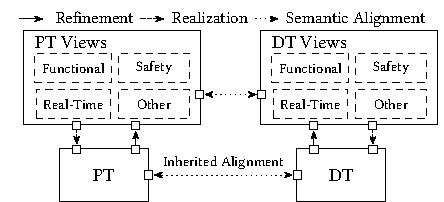
\includegraphics[width=0.45\textwidth]{figures/archi/fig_OCMPT_pdf.pdf}
\end{figure}
